\section{Berekening en fout viscsiteitsco\"effici\"ent $\eta$}

De viscositeitsco\"effici\"ent in het laminaire regime is
te berekenen aan de hand van de formule van Hagen-Poiseuille:
\begin{equation}
    \label{eq:hagen}
    Q = \frac{\pi \cdot \Delta P \cdot R^4}{8 \cdot L \cdot \eta}
\end{equation}
Deze formule is van de vorm $$y=a\cdot x$$ met de rico $a$ gelijk aan:
$$a = \frac{\pi \cdot R^4}{8 \cdot L \cdot \eta}$$
Door middel van deze formule berekent men $\eta$. \\

Deze $\eta$ zal men bepalen door een lineaire regressie toe te passen
op de gemeten waarden van het laminaire regime. We bevinden ons in
het geval van gelijkwaardige y-waarden.\\

Voor de lineaire regressie heeft men het principe der kleinste kwadraten
dat vereist dat de $\chi ^2$-vorm minimaal is: 
\begin{equation}
    \chi ^2 = \sum\limits_{i=1}^n(y_i-a\cdot x_i)^2
\end{equation}
De beste schatting voor de richtingco\"effici\"ent $a$ wordt gegeven door:
\begin{equation}
    \label{eq:a}
    \hat{a} \; \hat{=} \;\frac{\sum\limits_{i=0}^n x_i  y_i}{\sum\limits_{i=0}^n x_i^2}
\end{equation}
\begin{equation*}
    \hat{a} \; \hat{=} \; 6.31 \cdot 10^{-9}
\end{equation*}
Dus krijgt men de rechte:
$$Q = 6.31\cdot 10^{-9} \cdot \Delta P$$

Hiermee kan men de $\chi ^2$-vorm bepalen:
\begin{equation*}
    \chi ^2 = 1.31 \cdot 10^{-10}
\end{equation*}
Door bepaling van de standaardafwijking: 
\begin{equation}
    \sigma ^2 = \frac{\chi ^2}{n - 1}
\end{equation}
\begin{equation*}
    \sigma ^2 = 1.88 \cdot 10^{-11}
\end{equation*}
kan men de betrouwbaarheid op de richtingsco\"effici\"ent $a$ berekenen: 
\begin{equation}
    \label{eq:sa}
    \sigma ^2 \{ a \} = \frac{\sigma ^2}{\sum\limits_{i=1}^n x_i^2}
\end{equation}
\begin{equation*}
    \sigma ^2 \{ a \} =  5.70 \cdot 10^{-18}
\end{equation*}
Waardoor men voor $a$ het volgend resultaat bekomt:
$$a = 6.31 \cdot 10^{-9} \pm 5.70 \cdot 10^{-18}$$
Nu kunnen we uit formule \eqref{eq:hagen} viscositeitsco\"effici\"ent $\eta$ bepalen
\begin{equation*}
    \hat{\eta} = 9.89 \cdot 10^{-4}
\end{equation*}

Doordat $a$ een afschatting is en hiermee men $\eta$ berekent,
moet men ook de fout $\sigma ^2 \{ \eta \}$ bepalen

\begin{equation}
    \sigma ^2 \{ \eta \} = \left(\frac{\partial \hat{\eta}}{\partial \hat{a}}\right)^2 \cdot \sigma ^2 \{a\}
\end{equation}
\begin{equation*}
    \sigma ^2 \{ \eta \} = \left(\frac{\pi \cdot R^4}{8 \cdot L \cdot \hat{a^2}}\right)^2 \cdot \sigma ^2 \{a\}
\end{equation*}
Deze formule evalueren geeft:
\begin{equation*}
    \sigma \{ \eta \} = 1.40 \cdot 10^{-7}
\end{equation*}

met $a$ berekent in formule \eqref{eq:a} en $\sigma \{a\}$ in formule \eqref{eq:sa}

Ten slotte is de viscociteitsco\"effici\"ent gelijk aan:
\begin{equation*}
    \eta = (9.8909 \cdot 10^{-4} \pm 1.40 \cdot 10^{-7})Pa \cdot s
\end{equation*}

Nu alle waarden samengevat in een grafiek geeft:
\begin{figure}[H]
    \centering
    \caption{Grafiek laminaire en turbulente stroom}
    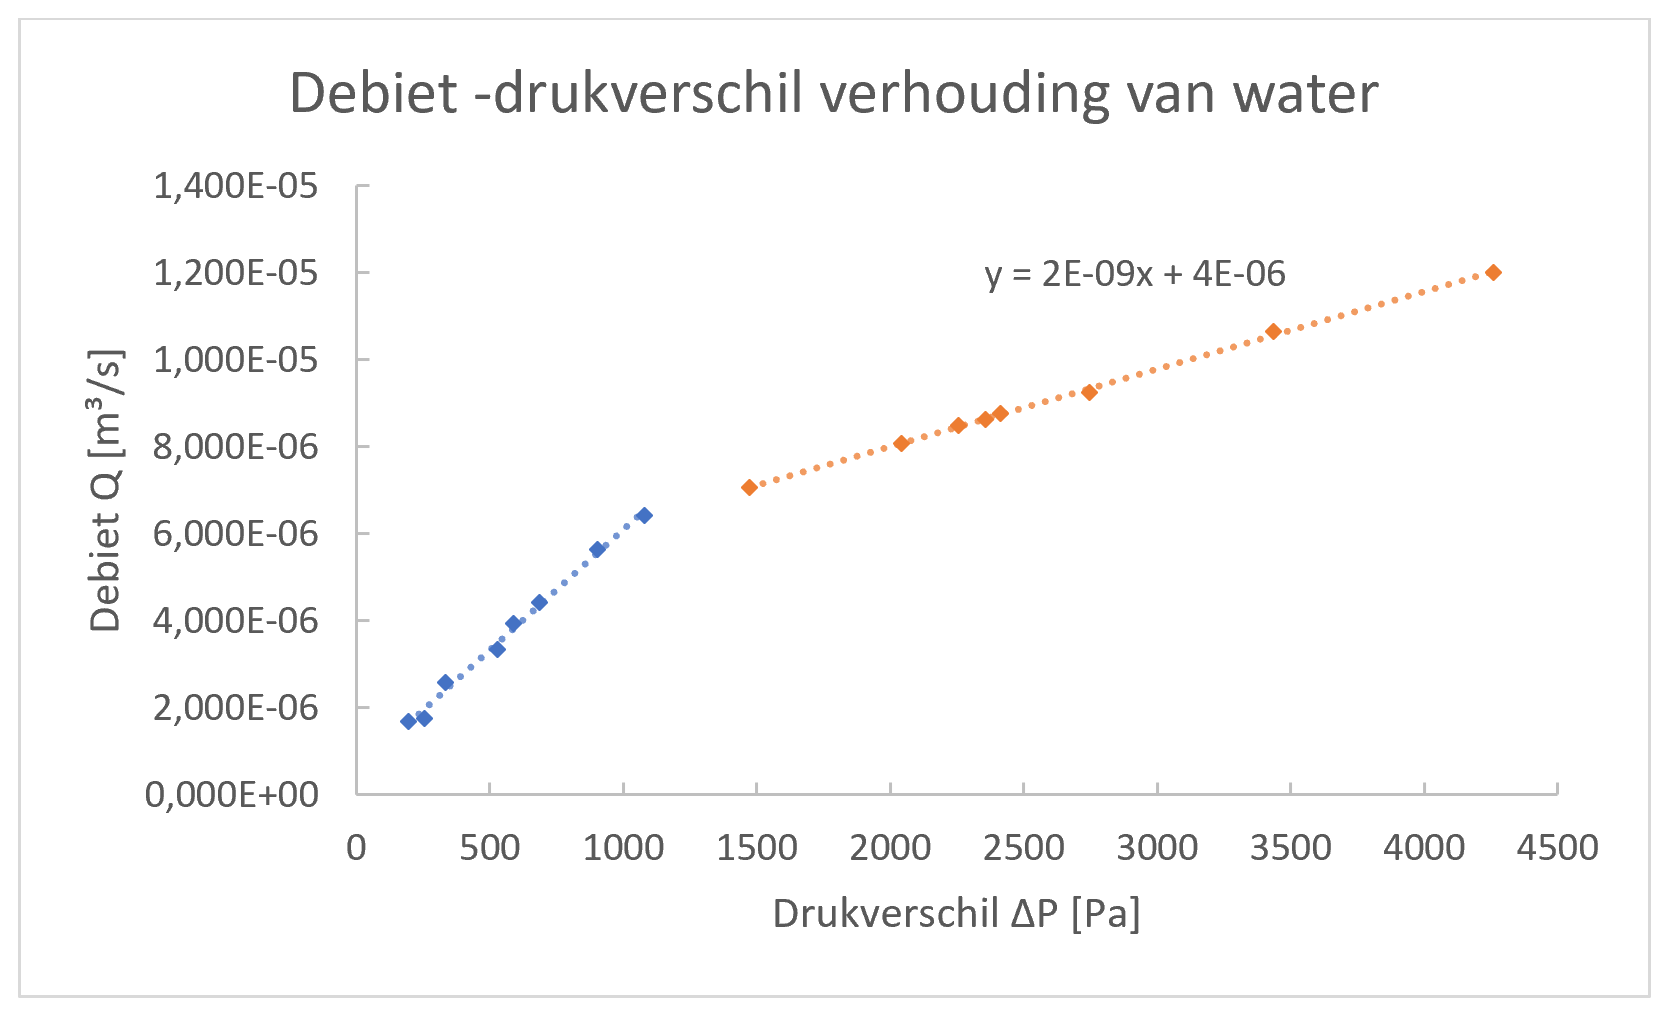
\includegraphics[width=0.8\textwidth]{img/grafiek.png}
    \label{fig:grafiek}
\end{figure}



